\documentclass[12pt]{report}

\usepackage{sty/DL_thesis_v2016}  % Global Style for particular SMU College, e.g. DL_thesis_v2016.sty

% \usepackage{DL_thesis_v2016}
\usepackage{adjustbox}       % TCM Extends the graphicx package to do trimming and other adjustments.
\usepackage{algorithm}       % TCM Algorithm block See http://algorithms.berlios.de/
\usepackage{algorithmic}     % TCM Algorithm & Peudocode See http://en.wikibooks.org/wiki/LaTeX/Algorithms_and_Pseudocode
\usepackage{amsmath}         % Need for subequations
\usepackage{mathrsfs} %https://ctan.org/pkg/mathrsfs
%\usepackage{amssymb}        % amssymb-telda and math symbols
\usepackage{booktabs}        % TCM Allows fancy Tables
\usepackage{boxedminipage}   % Boxes around figures
\usepackage{breqn}           % TCM Automatically breaks long equation lines - usually
\usepackage{changepage} 	 % TCM Allows one to temporarily change right and left margins
\usepackage{cite} 	 		 % TCM Allows improved handling of numeric citations including automatic ordering and ranges of multiple cites
\usepackage{enumitem} 		 % TCM Allows one to easily change the labels for enumerate list
%\usepackage{epsf}           % TCM This EPS file package is greatly depreciated for the graphicx package bundle. Use at own risk.
\usepackage{fancyhdr}
\usepackage{flafter}         % Floats should always appear after their definition
\usepackage[flushleft]{threeparttable}  % TCM This package allows for notes under tables.  Flushleft option flushes the note left margin of table (center is default)
\usepackage{geometry}		 % TCM Allows to customize paper size and margins.
\usepackage{graphicx}        % TCM Extends graphics package for figures. Provides op­tional ar­gu­ments to the \in­clude­graph­ics com­mand
\usepackage{epstopdf}        % TCM Converts eps images to PDF to use in graphicx package.  Must be loaded after graphicx package
\usepackage{longtable}       % TCM Allows for Automatic page breaks for long tables
%\usepackage{jneurosci}       % TCM The jneurosci bibliography style makes use of some commands - for example, \citeauthoryear.  Must include if using named or acmsmall bib style
\usepackage{ltablex}		 % TCM Modifies Tabularx Package by combining properties of tabularx and longtable.
\usepackage[maxfloats=36]{morefloats}      % Latex will handle more floats 18-36
\usepackage{moresize}        % TCM Adds \HUGE and \ssmall font sizes
\usepackage{multirow}        % TCM Allows multirow cells in tables (similar to merge and center in Excel)
%\usepackage{named}           % TCM Bibliography style that allows for more fine-tuned citing. Commands include \cite, \citeauthor, \citeyear and \shortcite (for after you've already used \citeauthor).
\usepackage{outlines}		 % TCM Needed for outlines
\usepackage{rotate}			 % TCM Performs rotations of floating environments (images w/ cations, etc)
\usepackage{rotating}        % Need for sidewaystable
\usepackage{scrextend}		 % TCM package that allows for KOMA-Script classes available for other classes: e.g., labeling lists etc.  See package documentation for further information.
\usepackage{pdflscape}		 % TCM Allows Landscape Page
%%\usepackage{qtree}         % Need for trees
\usepackage{setspace}        % TCM Allows for more intuitive commands for single and double spacing
\usepackage{siunitx}		 % TCM package required to ensure units are typeset properly with numbers e.g. \SI{10}{\kg\m\per\square\s}
\sisetup{output-exponent-marker=\ensuremath{\mathrm{E}}}  % TCM Option allows for Scientific notation of Numbers.  Format is \num{#.####E##}
% \usepackage[superscript]{cite}		  % TCM Makes citations superscript instead of [#]
\usepackage [table]{xcolor}	 % TCM Allows coloring of tables
\usepackage{tabularx}		 % TCM Package which allows paragraphs in Tables
% \usepackage{thumbpdf}		  % TCM Comment out as causes warnings, can easily create thumbs in Adobe if needed.

%===========================================================
%  Color ToDo Comment Notes for editing
%===========================================================
\usepackage[colorinlistoftodos,textwidth=25mm,shadow,backgroundcolor=green]{todonotes}				  % TCM Allows margin comments
\usepackage{marginnote}				  % TCM Require for Todonotes in Align Envionment
%~~~~~~~~~~~~~~~~~~~~~~~~~~~~~~~~~~~~~~~~~~~~~~~~~~~~~~~~~~~
% TCM  BEGIN Altering Todonotes Commands to use Marginnote instead of Marginpar to use todonotes in align environment
%~~~~~~~~~~~~~~~~~~~~~~~~~~~~~~~~~~~~~~~~~~~~~~~~~~~~~~~~~~~
\makeatletter
\renewcommand{\@todonotes@drawMarginNoteWithLine}{%
 \begin{tikzpicture}[remember picture, overlay, baseline=-0.75ex]%
  \node [coordinate] (inText) {};%
 \end{tikzpicture}%
 \marginnote[{% Draw note in left margin
  \@todonotes@drawMarginNote%
  \@todonotes@drawLineToLeftMargin%
  }]{% Draw note in right margin
  \@todonotes@drawMarginNote%
  \@todonotes@drawLineToRightMargin%
 }%
}
\makeatother
%----------------------------------------------------
% TCM  BEGIN New Todonotes Command to use single line spacing (sls) in note
%----------------------------------------------------
\newcommand{\slstodo}[2][]
{\todo[caption={#2}, size=\small, #1]{\renewcommand{\baselinestretch}{0.5}\selectfont#2\par}}
%----------------------------------------------------
% TCM  END New Todonotes Command to use single spacing in note
%----------------------------------------------------

%~~~~~~~~~~~~~~~~~~~~~~~~~~~~~~~~~~~~~~~~~~~~~~~~~~~~~~~~~~~
% TCM  END Altering Todonotes Commands to use Marginnote instead of Marginpar to use todonotes in align
%~~~~~~~~~~~~~~~~~~~~~~~~~~~~~~~~~~~~~~~~~~~~~~~~~~~~~~~~~~~

\usepackage{verbatim}        % TCM Verbatim text block
\usepackage{wrapfig}         % Wrap figures
\usepackage{xspace}          % Allows dynamic space in global text variables. This can allow you to just use \newCommandName rather than \newCommandName{}.
\usepackage [bookmarks=true,backref=page, hyperfigures=true, pdfpagelabels=false] {hyperref}
\hypersetup{
 % TCM Added more precise definition and options for Hyperref package.
 % TCM Comment out or change hyperref preferences
 % TCM \hypersetup should be loaded last
 bookmarksopen=true,				  % True: Open bookmark tree
 bookmarksnumbered=true, 		  % True: put section numbers in bookmarks
 breaklinks=true,				  % True: split the url over multiple lines
 %    draft=true,						  % True: do not do any hyper linking
 filecolor=magenta, 				  % Color of file links
 citecolor=blue, 				  % Color of links to bibliography
 colorlinks=true, 				  % False: boxed links; true: colored links
 linkcolor=blue, 				  % Color of internal links
 linktocpage=true, 				  % True: Makes the page number of TOC the link vs the text
 %    pagebackref=true,				  % True: Links references back to referring page
 pdfnewwindow=true,         		  % True: URL links in new window
 plainpages=false, 				  % True: do page number anchors as plain Arabic
 pdffitwindow=false,        		  % Window fit to page when opened
 pdfmenubar=true,           		  % Show Acrobat menu
 pdfstartview={FitH},       		  % Fits the width of the page to the window
 pdftoolbar=true, 				  % Show Acrobat toolbar
 pdfauthor={Author}, 			  % Author in PDF document properties
 pdfcreator={Author}, 			  % Creator of the document in PDF document properties
 pdfkeywords={Keyword1} {Keyword2} {Keyword3} {Keyword4} {Author}, % List of keywords in PDF document properties
 pdfproducer={Producer}, 		  % Producer of the document in PDF document properties
 pdfsubject={Subject},   % Subject of the document in PDF document properties
 pdftitle={Title of Dissertation}, % Title in PDF document properties
 unicode=false,             		  % Non-Latin characters in Acrobat bookmarks
 urlcolor=cyan 					  % Color of external links
}
\usepackage{bookmark}		 		  % TCM Eliminates Warning Bookmark level greater than one.  Must be loaded after Hyperref


\geometry{letterpaper, margin=1in} % Dedman/Lyle Standard 2016

\linespread{1.6}
\setcounter{secnumdepth}{4} % Sets number subsections
\setcounter{tocdepth}{4}    % Set the number of subsections in TOC

\urlstyle{same} % Set URL style to same font as text verses mono-spaced, i.e., courier

%======================================================================
% Custom Commands  Inital Creation TCM 2015
%======================================================================
% Use this document to place all of your global new commands
%======================================================================

%======================================================================
% BEGIN SMU Custom Commands
%======================================================================
% The many of the following commands were originally in the smu_thesis.sty
% file. Commands and comments were moved here to make style file more about
% document style. While custom environments can technically be considered 
% style, the student created environments are included here to simplify
% the style file. Often these commands were created by students over the
% years and placed in the style file.  The commands have not been 
% verified and can be obsolete LaTeX commands. The Commands can be used 
% or ignored. 
%======================================================================
%----------------------------------------------------------------------
% BEGIN TCM Commands to set formatting for Paragraph section to have line
%           feed after heading & Numbered. This custom command makes
%           \paragraph, in essence, a form of \subsubsubsection.
%           Uncomment to use.
%----------------------------------------------------------------------
%  \makeatletter
%  \renewcommand\paragraph{\@startsection{paragraph}{4}{\z@}%
%    {-3.25ex\@plus -1ex \@minus -.2ex}%
%    {1.5ex \@plus .2ex}%
%    {\normalfont\normalsize\bfseries}}
%  \makeatother
%----------------------------------------------------------------------
% END of Commands to set formatting for Paragraph section to have line
%       feed after heading TCM
%----------------------------------------------------------------------
%----------------------------------------------------------------------
% BEGIN Shortcuts to insert calligraphic letters in Math Mode Only
%----------------------------------------------------------------------
\newcommand{\cA}{{\mathcal A}}
\newcommand{\cB}{{\mathcal B}}
\newcommand{\cC}{{\mathcal C}}
\newcommand{\cD}{{\mathcal D}}
\newcommand{\cE}{{\mathcal E}}
\newcommand{\cF}{{\mathcal F}}
\newcommand{\cG}{{\mathcal G}}
\newcommand{\cH}{{\mathcal H}}
\newcommand{\cI}{{\mathcal I}}
\newcommand{\cJ}{{\mathcal J}}
\newcommand{\cK}{{\mathcal K}}
\newcommand{\cL}{{\mathcal L}}
\newcommand{\cM}{{\mathcal M}}
\newcommand{\cN}{{\mathcal N}}
\newcommand{\cO}{{\mathcal O}}
\newcommand{\cP}{{\mathcal P}}
\newcommand{\cQ}{{\mathcal Q}}
\newcommand{\cR}{{\mathcal R}}
\newcommand{\cS}{{\mathcal S}}
\newcommand{\cT}{{\mathcal T}}
\newcommand{\cU}{{\mathcal U}}
\newcommand{\cV}{{\mathcal V}}
\newcommand{\cW}{{\mathcal W}}
\newcommand{\cX}{{\mathcal X}}
\newcommand{\cY}{{\mathcal Y}}
\newcommand{\cZ}{{\mathcal Z}}
% Lower case caligraphy letters
\newcommand{\cw}{{\mathcal w}}
%----------------------------------------------------------------------
% END Shortcuts to insert calligraphic letters in Math Mode Only
%----------------------------------------------------------------------
%----------------------------------------------------------------------
% BEGIN Shortcuts to insert boldface letters 
%----------------------------------------------------------------------
\newcommand{\bA}{{\bf A}}
\newcommand{\bB}{{\bf B}}
\newcommand{\bC}{{\bf C}}
\newcommand{\bD}{{\bf D}}
\newcommand{\bE}{{\bf E}}
\newcommand{\bF}{{\bf F}}
\newcommand{\bG}{{\bf G}}
\newcommand{\bH}{{\bf H}}
\newcommand{\bI}{{\bf I}}
\newcommand{\bJ}{{\bf J}}
\newcommand{\bK}{{\bf K}}
\newcommand{\bL}{{\bf L}}
\newcommand{\bM}{{\bf M}}
\newcommand{\bN}{{\bf N}}
\newcommand{\bO}{{\bf O}}
\newcommand{\bP}{{\bf P}}
\newcommand{\bQ}{{\bf Q}}
\newcommand{\bR}{{\bf R}}
\newcommand{\bS}{{\bf S}}
\newcommand{\bT}{{\bf T}}
\newcommand{\bU}{{\bf U}}
\newcommand{\bV}{{\bf V}}
\newcommand{\bW}{{\bf W}}
\newcommand{\bX}{{\bf X}}
\newcommand{\bY}{{\bf Y}}
\newcommand{\bZ}{{\bf Z}}
%----------------------------------------------------------------------
% END Shortcuts to insert boldface letters 
%----------------------------------------------------------------------
%----------------------------------------------------------------------
% BEGIN Shortcuts to insert overline symbols in Math Mode Only
%----------------------------------------------------------------------
\newcommand{\oA}{{\overline A}}
\newcommand{\oB}{{\overline B}}
\newcommand{\oC}{{\overline C}}
\newcommand{\oD}{{\overline D}}
\newcommand{\oE}{{\overline E}}
\newcommand{\oF}{{\overline F}}
\newcommand{\oG}{{\overline G}}
\newcommand{\oH}{{\overline H}}
\newcommand{\oI}{{\overline I}}
\newcommand{\oJ}{{\overline J}}
\newcommand{\oK}{{\overline K}}
\newcommand{\oL}{{\overline L}}
\newcommand{\oM}{{\overline M}}
\newcommand{\oN}{{\overline N}}
\newcommand{\oO}{{\overline O}}
\newcommand{\oP}{{\overline P}}
\newcommand{\oQ}{{\overline Q}}
\newcommand{\oR}{{\overline R}}
\newcommand{\oS}{{\overline S}}
\newcommand{\oT}{{\overline T}}
\newcommand{\oU}{{\overline U}}
\newcommand{\oV}{{\overline V}}
\newcommand{\oW}{{\overline W}}
\newcommand{\oX}{{\overline X}}
\newcommand{\oY}{{\overline Y}}
\newcommand{\oZ}{{\overline Z}}
% Lower case overline
\newcommand{\ovd}{{\overline d}}
\newcommand{\ove}{{\overline e}}
\newcommand{\ovf}{{\overline f}}
\newcommand{\ovg}{{\overline g}}
\newcommand{\ovh}{{\overline h}}
\newcommand{\ovi}{{\overline i}}
%----------------------------------------------------------------------
% END Shortcuts to insert overline symbols in Math Mode Only
%----------------------------------------------------------------------
%----------------------------------------------------------------------
% BEGIN Shortcuts to insert vector symbols in Math Mode Only
%----------------------------------------------------------------------
\newcommand{\vS}{{\vec S}}
\newcommand{\vT}{{\vec T}}
\newcommand{\vU}{{\vec U}}
\newcommand{\vV}{{\vec V}}
\newcommand{\vW}{{\vec W}}
\newcommand{\vX}{{\vec X}}
\newcommand{\vY}{{\vec Y}}
\newcommand{\vZ}{{\vec Z}}
% Lower case vectors
\newcommand{\vs}{{\vec s}}
\newcommand{\vt}{{\vec t}}
\newcommand{\vu}{{\vec u}}
\newcommand{\vv}{{\vec v}}
\newcommand{\vw}{{\vec w}}
\newcommand{\vx}{{\vec x}}
%----------------------------------------------------------------------
% END Shortcuts to insert vector symbols in Math Mode Only
%----------------------------------------------------------------------
%----------------------------------------------------------------------
% BEGIN Misc. Commands defined by students
%----------------------------------------------------------------------
\newcommand{\myqed}{\vspace{-1.1cm} \qed \vspace{0.9cm}}
\newcommand{\qed}{\mbox{$\ \Box$}}
\newcommand{\lqed}{\qed\vspace{.1in}}
\newcommand{\nf}{{\mbox{$\sim$}}}
\newcommand{\wt}{\mbox{$\widehat{T}$}}
\newcommand{\as}{\mbox{$/\hspace{-2mm}>$}}
\newcommand{\equi}{\mbox{$\leftrightarrow$}}
\newcommand{\myeq}{\mbox{$\leftrightarrow$}}
%\newcommand{\tab}{\hspace*{4em}}
%\newcommand{\ind}{\hspace*{2em}}
%\newcommand{\mif}{\mbox{ :- }}
%\newcommand{\dd}{\mbox{$\bullet$}}
\newcommand{\dd}{\mbox{\ $\mid$\ }}

\newcommand{\ind}{\hspace*{2.0em}}
\newcommand{\tab}{\hspace*{4em}}

\newcommand{\myp}{\protect{$+$}}
\newcommand{\mypp}[1]{\protect{${#1}$}}
\newcommand{\myf}[2]{\protect{\ \(\frac{\mbox{\rm #1}}{\mbox{\rm #2}}\)}\ }
\newcommand{\myup}{\protect{$ \uparrow$}}
\newcommand{\scc}[1]{\protect{\ \ \ $ SCC = {#1} $}}

\newcommand{\twoheadrightarrow}{{\rightarrow \hspace{-0.3cm} \rightarrow \hspace{0.2cm}}}

\newcommand{\chap}[1]{\chapter{\protect{\bf {#1}}}}
\newcommand{\mytab}{\hspace*{13em}}
\newcommand{\bleft}{\left \{\ }
\newcommand{\bright}{\ \right \}}
\newcommand{\sind}{ \ \ \ }
\newcommand{\mand}{ \ \&\ }
\newcommand{\mif}{\mbox{\ :-\ }}
%%%\newcommand{\nf}{\sim}
\newcommand{\posI}{$I^+$}
\newcommand{\negI}{$I^-$}
%\newcommand{\AST}{$AST(P)$}
\newcommand{\Ip}[1]{${\mathcal I}_{#1}$}
\newcommand{\II}[1]{${\mathcal I}({#1})$}
%\newcommand{\HU}[1]{${\mathcal HU}_{#1}$}
%\newcommand{\US}{${\mathcal US}$}
%\newcommand{\HB}[1]{${\mathcal HB}_{#1}$}
%----- chen  -----------------
%\newcommand{\emptyset}{\phi}
\newcommand{\cUS}{{\mathcal US}}
\newcommand{\cHU}{{\mathcal HU}}
\newcommand{\cHB}{{\mathcal HB}}
\newcommand{\cUC}{{\mathcal UC}s}
\newcommand{\cBody}{{\mathcal B}ody}
\newcommand{\wA}{\widetilde{\rm A}}
\newcommand{\LF}{${\mathcal LF}$}
\newcommand{\DI}{DI^+ \cup DI^-}
\newcommand{\AI}{AI^+ \cup AI^-}
\newcommand{\Asp}{\tt asp}
\newcommand{\Aspt}[1]{${\tt asp}({#1})$}
\newcommand{\BP}[1]{${\mathcal BP}({#1})$}
\newcommand{\myarrow}{-\hspace*{-0.23cm}-\hspace*{-0.23cm}-\hspace*{-0.23cm}\longrightarrow}
\newcommand{\nedge}{\rightarrow\hspace*{-0.39cm}{\prime} \hspace*{0.29cm}}
\newcommand{\jmp}[1] {\hspace*{0.3in}{#1}\hspace*{0.3in}}
\newcommand{\Aro}[1]{\stackrel{#1}\longrightarrow}
\newcommand{\MyAro}[1]{\stackrel{#1}\myarrow}
\newcommand{\MyLoAro}[1]{\stackrel{#1}{-\hspace*{-0.23cm}-\hspace*{-0.23cm}\myarrow}}

%----- For figures  ---------------------------------------------------

\newcommand{\myfigureold}[3]{ \begin{figure}[tbp]
  \begin{center}
   \fbox{
    \begin{minipage}[t]{5.7in}
    \rule[-.1cm]{0cm}{0.5cm} % changed by saeed to 0.01cm was 0.5cm
    \centerline{\psfig{#1}}
    \end{minipage}
    }
    \end{center}
       \caption{#2} \label{#3} \vskip -0.14in \end{figure} } % changed by saeed was -0.14 changed to -0.01in

\newcommand{\mytabfig}[3]{ \begin{figure}[tbp]
  \begin{center}
   \fbox{
    \begin{minipage}[t]{5.7in}
    \rule[-.1cm]{0cm}{0.5cm} % changed by saeed to 0.01cm was 0.5cm
#1
    \end{minipage}
        }
        \end{center}
       \caption{#2} \label{#3} \vskip -0.14in \end{figure} } % changed by saeed was -0.14 changed to -0.01in

\newcommand{\myfigure}[3]{ \begin{figure}[tbp]
    \begin{center}
    #1
    \end{center}
    \caption{#2} \label{#3} \vskip -0.14in \end{figure} } % changed by saeed was -0.14 changed to -0.01in

\newcommand{\mytable}[3]{ \begin{table}[tbp]
  \begin{center}
  \caption{#2}
    #1
  \label{#3} \vskip -0.01in \end{center} \end{table} }

\newcommand{\myendfig}{\vskip -0.14in \end{figure} } % changed by saeed was -0.14in changed to -0.01in
\newcommand{\myendtab}{\vskip -0.01in \end{table} }

%----------------- theorem definitions --------------------------------

\newtheorem{ex}{Example}[chapter]
\newtheorem{theor}{Theorem}[chapter]
\newtheorem{mtd}{Method}[chapter]
\newtheorem{mydef}{Definition}[chapter]
%\newtheorem{mylem}{Lemma}[chapter]
\newtheorem{mylem}[theor]{Lemma}

%\newtheorem{algorithm}{Algorithm}[chapter]
%\newtheorem{corollary}[theorem]{Corollary}
%\newtheorem{proposition}{Proposition}[section]
%\newtheorem{remark}{Remark}[section]

%----------------------------------------------------------------------
%\font\pf=rpcrr at 11pt    % TCM Comment out if using Overleaf.com
%\font\spf=rpcrr at 11pt   % TCM Comment out if using Overleaf.com
%----------------------------------------------------------------------

%-------------------- environment definitions -------------------------
\newenvironment{example}{\begin{ex} \rm}{\hfill \qed \end{ex}}
\newenvironment{theorem}{\begin{theor}}{ \end{theor}}
\newenvironment{method}{\begin{mtd} \rm}{\hfill \qed \end{mtd}}
\newenvironment{definition}{\begin{mydef} \rm}{\hfill \qed \end{mydef}}
%\newenvironment{lemma}{\begin{mylem} \rm}{\hfill \qed \end{mylem}}
\newenvironment{lemma}{\begin{mylem}}{ \end{mylem}}

\newenvironment{vers}{\vspace{-0.1cm} \begin{verse}}{\vspace{-0.1cm} \end{verse}}
\newenvironment{vers2}{\vspace{-0.2cm} \begin{verse}}{\vspace{-0.1cm} \end{verse}}

\newenvironment{proof}[0]{\vspace{0.3cm}\noindent {\bf Proof:} \rm }{\hfill \lqed}
\newenvironment{proof-of}[1]{\noindent {\bf Proof of #1:}}{\hfill \lqed}
%----------------------------------------------------------------------
% END Misc. Commands defined by students
%----------------------------------------------------------------------
%======================================================================
% END SMU Custom Commands
%======================================================================

%-----------------------------------------------------------
%  Reduce compile warnings for overfull and underfull hboxes & vboxes
%       Adjust up or down to fit your specific needs
%-----------------------------------------------------------
\hbadness=50000
\vbadness=50000
\hfuzz=150pt
%-----------------------------------------------------------
% Reduce compile warnings for overfull and underfull hboxes
%-----------------------------------------------------------
%-----------------------------------------------------------
% eliminate compile warnings for noindent hfill hbox in PDF bookmarks
%-----------------------------------------------------------
\pdfstringdefDisableCommands{
\def\hbox{ }% hyperref (temporarily) changes \hbox to a space in this context.
\def\hfill{ }% hyperref (temporarily) changes \hfill to a space in this context.
\def\noindent{ }% hyperref (temporarily) changes \noindent to a space in this context.
\def\hskip{ }% hyperref (temporarily) changes \hskip to a space in this context.
}

% \thesisdraft % uncomment if want draft printing

\begin{document}

%======================================================================
% Front Pages  Initial Creation TCM 2015
%======================================================================
% This file sets up the initial pages of the thesis/dissertation/praxis
% Change all the sample information for your specific document.
%======================================================================

%----------------------------------------------------------------------
%%  Last name, First name, Initial
%----------------------------------------------------------------------
\Name{Feickert}{Matthew}{} % Don't put anything in the last brackets

%----------------------------------------------------------------------
% Title -- you have up to three lines to specify your title each line
% should be no more than 48 characters long
%----------------------------------------------------------------------
\Title{A Search for Higgs Bosons decaying to the $\MakeLowercase{b}\bar{\MakeLowercase{b}}$ Final State}{Through Production with An Initial State Radiation Jet}{using the ATLAS Detector at $\sqrt{\MakeLowercase{s}}=\SI{13}{\tera\electronvolt}$}

%----------------------------------------------------------------------
% Previous Earned Degrees
%----------------------------------------------------------------------
\DegreeA{B.S., Engineering Physics, University of Illinois at Urbana-Champaign}
\DegreeB{M.A., Physics, University of Virginia}
\DegreeC{M.S., Physics, Southern Methodist University}


%----------------------------------------------------------------------
% Degree you are seeking
%----------------------------------------------------------------------
\DegreeSought{Doctor of Philosophy}

%----------------------------------------------------------------------
% Major of the degree you are seeking
%----------------------------------------------------------------------
\Major{Physics}

\University{Southern Methodist University}

%----------------------------------------------------------------------
% School from which the degree will be from
%----------------------------------------------------------------------
\School{Dedman College}

%----------------------------------------------------------------------
% Date the degree will be conferred
%----------------------------------------------------------------------
\DegreeDate{May 14, 2019}

%----------------------------------------------------------------------
% Date the thesis will be defended
%----------------------------------------------------------------------
\ThesisDate{April 17, 2019}


%----------------------------------------------------------------------
% Is this a thesis, dissertation, or something else?
%----------------------------------------------------------------------
\ThesisType{Dissertation}

%----------------------------------------------------------------------
% Your Committee
%----------------------------------------------------------------------
\Advisor{Dr.~Stephen Sekula}
\AdvisorTitle{Associate Professor}

\CommitteeMemberA{Dr.~Jingbo Ye}
\CommitteeMemberTitleA{Professor}

\CommitteeMemberB{Dr.~Roberto Vega}
\CommitteeMemberTitleB{Associate Professor}

\CommitteeMemberC{Dr.~TBA}
\CommitteeMemberTitleC{Assistant Professor}

% \CommitteeMemberD{}           % Uncomment if needed
% \CommitteeMemberTitleD{}      % Uncomment if needed


%===================================================================
%   Create the front pages of the thesis
%===================================================================

\ApprovalTitlePages

\Copyright% TCM Copyright Page per Dedman 2016 Standards

%----------------------------------------------------------------------
% Include your acknowledgments
% If no dedication, move Acknowledgment to where dedication is and add to
% Table of contents
%----------------------------------------------------------------------
% \addcontentsline{toc}{chapter}{\protect \noindent {ACKNOWLEDGMENTS}}
\begin{Acknowledgment}
 Acknowledgments text goes here.

\end{Acknowledgment}

%----------------------------------------------------------------------
% Include your abstract
%----------------------------------------------------------------------
\begin{Abstract}
 Abstract text goes here.

\end{Abstract}

\PreliminaryPages

%----------------------------------------------------------------------
% Need a List of Symbols Page?
%----------------------------------------------------------------------
% Uncomment to insert a list of symbols from symbols.tex (or elsewhere)
%\begin{listofsymbols}
%\input{symbols}
%\end{listofsymbols}

%----------------------------------------------------------------------
% Include your dedication
%----------------------------------------------------------------------
\Dedicate{Dedication text goes here}


\begin{thesis}

 \chapter*{Preface}\label{chapter:preface}
% c.f. https://tex.stackexchange.com/a/222961/152544
\addcontentsline{toc}{chapter}{\protect\numberline{}Preface}

The following is a summary of useful concepts in high energy particle physics.

\section{Units}\label{section:units}

\subsection{Natural Units}\label{subsection:natural_units}

The nature of high energy physics is to give descriptions of the phenomena and interactions that occur at energies that result in speeds that are close to the speed of light over very short time and distance scales.
Given this, it becomes readily apparent that International System of Units (SI) of measurement are somewhat cumbersome to use in calculations, and a much more useful system of units would be consistent with the scale of the phenomena.
When measuring the speed of a relativistic particle it is more convenient to compare to the speed of light $\left(\text{such that }c=1\right)$ then to the number of meters per second.
Similarly, when measuring the momentum of a particle it is generally more useful to know the amount of its energy in the form of momentum compared to the amount in the form of its mass, resulting in expressing momentum in terms of energy.
This system of units is called ``Natural Units'', and builds its measurements in terms of speed, angular momentum, and energy.
It is used extensively (if not almost exclusively) throughout high energy physics.
Quantities encountered routinely in high energy physics are given in Natural Units in \Cref{table:natural_units}.
\TODO{Describe cross section.}

\begin{table}[htpb]
 \centering
 \caption{Common quantities in particle physics given in both natural units and SI units.}
 \begin{tabular}{@{}llll@{}} \toprule
  Quantity         & Natural Units                 & Natural Units (dimensionful)            & SI Units                                              \\ \midrule
  Speed            & $1$                           & $c$                                     & $3.0\times 10^{8}~\mathrm{m}/\mathrm{s}$              \\
  Angular Momentum & $1$                           & $\hbar$                                 & $10^{34}~\mathrm{m}^2 \,\mathrm{kg}/\mathrm{s}$       \\
  Energy           & $\mathrm{GeV}$                & $\mathrm{GeV}$                          & $1.6\times 10^{-10}~\mathrm{J}$                       \\
  Momentum         & $\mathrm{GeV}$                & $\mathrm{GeV}/c$                        & $1\times 10^{-19}~\mathrm{kg}\,\mathrm{m}/\mathrm{s}$ \\
  Mass             & $\mathrm{GeV}$                & $\mathrm{GeV}/c^{2}$                    & $1.8\times 10^{-27}~\mathrm{kg}$                      \\
  Time             & $1/\mathrm{GeV}$              & $\hbar/\mathrm{GeV}$                    & $6.6\time 10^{-25}~\mathrm{s}$                        \\
  Length           & $1/\mathrm{GeV}$              & $\hbar c/\mathrm{GeV}$                  & $2\times 10^{-16}~\mathrm{m}$                         \\
  Electric Charge  & $1$                           & $e/\sqrt{4\pi \alpha_{\mathrm{em}}}$    & $5.3\times 10^{-19}~\mathrm{C}$                       \\
  Magnetic Field   & $\left(\mathrm{GeV}\right)^2$ & $\left(\mathrm{GeV}\right)^2/\hbar c^2$ & $5\times 10^{16}~\mathrm{T}$                          \\
  \bottomrule
 \end{tabular}\label{table:natural_units}%
\end{table}


\subsection{Units of Luminosity}\label{subsection:luminosity_units}
In high energy physics a crucial quantity of interest is the luminosity (both instantaneous and integrated) delivered by the particle accelerator.
The instantaneous luminosity, $\mathscr{L}$, can be defined as the number of particles incident per unit area per unit time (generally taken to be seconds),
\begin{equation}
 \mathscr{L} = \frac{\text{number of particles}}{\text{unit area} \cdot \text{second}}.
 \label{eq:instantaneous_luminosity}
\end{equation}
In accelerator physics, the unit area is generally chosen to be $\textrm{cm}^2$, giving instantaneous luminosities units of $\textrm{cm}^{-2} \cdot \textrm{s}^{-1}$,
\[
 \left[\mathscr{L}\right] = \textrm{cm}^{-2} \cdot \textrm{s}^{-1}.
\]
However, experimental particle physicists prefer to use units of inverse barns for luminosities. A barn is defined as
\begin{equation}
 1~\textrm{barn} = 10^{-28}~\textrm{m}^2 = 10^{-24}~\textrm{cm}^2,
 \label{eq:barn_to_area}
\end{equation}
which is roughly the cross sectional area of an atomic nuclei~\cite{web:history_physics_purdue,history:etymology_barn}.

The context in which luminosity appears as being useful is in the form of an equation like
\begin{equation}
 N_{\textrm{events}} = \sigma_{\textrm{process}} \cdot \int \mathscr{L}\,dt
 \label{eq:events_from_luminosity}
\end{equation}
where:
\begin{itemize}
 \item $N_{\text{events}}$ is the number of events of a particular process that will be produced at the collider.
       This is what ends up exiting the collision process.
 \item $\sigma_{\textrm{process}}$ is the cross section of the particular process to occur per interaction of colliding particles.
       At the \Gls{LHC} this would be the cross section per proton-proton interaction.
       This is a function of the fundamental physics that is available at the energy ranges being probed, and so is also a function of the collider's center of mass energy, $\sqrt{s}$.
       When written in an equation as such it is assumed that the cross section is also including the relevant branching ratios for the final state particles.
       That is, $\sigma\left(pp \to H \to b\bar{b}\,\right) = \sigma\left(pp \to H\right) \cdot \mathcal{BR}\left(H \to b\bar{b}\,\right)$.
 \item $L \equiv \int \mathscr{L}\,dt$ is the total luminosity integrated over time (the integrated luminosity).~\cite{Herr:941318}
       This is what is delivered by the particle accelerator.
\end{itemize}

\begin{table}[htpb]
 \centering
 \caption{Instantaneous luminosities at the LHC.}
 \begin{tabular}{@{}ll@{}} \toprule
  Description                                                    & Units of $\textrm{cm}^{-2}\cdot\textrm{s}^{-1}$ \\ \midrule
  LHC Design Luminosity~\cite{Bruning:782076}                    & $10^{34}$                                       \\
  2017 ATLAS Trigger Menu Maximum~\cite{TWiki:MenuEvolution2017} & $2.0 \times 10^{34}$                            \\
  2017 Plan~\cite{Indico:MenuCoordination_2017Lumi}              & $1.7 \times 10^{34}$                            \\
  2017 Peak~\cite{TWiki:2017ATLASPeakLumi}                       & $20.9 \times 10^{33}$                           \\
  2018 Peak~\cite{TWiki:2018ATLASPeakLumi}                       & $21.0 \times 10^{33}$                           \\
  \bottomrule
 \end{tabular}\label{table:LHC_Luminosity_Goals}%
\end{table}

% Note to self: spacing in tables seems too large. See if can adjust with geometry package
\begin{table}[htpb]
 \centering
 \caption{Luminosity measurements in $\text{barns}^{-1}$.}
 % \resizebox{\linewidth}{!}{%
 % \resizebox*{!}{\dimexpr\textheight-2\baselineskip\relax}{%
 \begin{tabular}{@{}lll@{}} \toprule
  Units                & Units of $\textrm{cm}^{-2}$ & Units of $\textrm{fb}^{-1}$ \\ \midrule
  $\textrm{barn}^{-1}$ & $10^{24}$                   & $10^{-15}$                  \\
  $\textrm{mb}^{-1}$   & $10^{27}$                   & $10^{-12}$                  \\
  $\mu\textrm{b}^{-1}$ & $10^{30}$                   & $10^{-9}$                   \\
  $\textrm{nb}^{-1}$   & $10^{33}$                   & $10^{-6}$                   \\
  $\textrm{pb}^{-1}$   & $10^{36}$                   & $10^{-3}$                   \\
  $\textrm{fb}^{-1}$   & $10^{39}$                   & $10^{0}$                    \\
  $\textrm{ab}^{-1}$   & $10^{42}$                   & $10^{3}$                    \\
  \bottomrule
 \end{tabular}\label{table:Luminosity}%
 % }
\end{table}

\section{Coordinates}\label{section:coordinates}

LHC coordinate systems\\

The LHC coordinate system, seen in \Cref{fig:LHC_coordinate_system}, is a rectangular coordinate system defined relative to the LHC ring and the LHC beamline.
At any point, the positive $x$ direction is defined as the direction that points radially inward to the center of the LHC ring.
The positive $y$ direction is then defined as pointing upwards --- towards the Earth's surface if one is at the beamline --- leaving the positive $z$ direction pointing along the beamline.

\begin{figure}[htbp]
 \centering
 \includegraphics{preface/LHC_coordinate_system.pdf}
 \caption{The LHC coordinate system as seen from the ATLAS detector.}
 \label{fig:LHC_coordinate_system}
\end{figure}

While the LHC coordinate system is Cartesian, the preferred coordinate system for describing LHC events is not.
As the ATLAS detector is arranged cylindrically outside the beamline of the LHC --- such that most of its detector components are transverse to the beamline --- the coordinate system that is used to describe events in ATLAS is characterized by a particle's transverse momentum, pseudorapidity, and polar angle: $\left(p_T, \eta, \theta\right)$.
The polar angle, $\theta$, is defined as the angle relative to the beam axis, and the azimuthal angle, $\phi$, is measured around the beam axis.

\Gls{Pseudorapidity} is defined as
\begin{equation}
 \eta = - \ln \left(\tan \frac{\theta}{2}\right)
 \label{eq:pseudorapidity}
\end{equation}
to be a good approximation in the high energy regime of the \gls{rapidity} of a particle --- a measurement of the velocity of a particle longitudinal to the beam axis,
\begin{equation}
 y = \frac{1}{2} \ln \left(\frac{E + p_{z}}{E - p_{z}}\right).
 \label{eq:rapidity}
\end{equation}
As the beam axis is defined as $\hat{\vec{z}}$, such that $p_{z} = \abs{\vec{p}} \cos\theta$, then it is seen that in the relativistic limit, $\abs{\vec{p}} \gg m$, the rapidity reduces to the pseudorapidity
\[
 \begin{split}
  y   &\approx \frac{1}{2} \ln \left(\frac{p + p\cos\theta}{p - p\cos\theta}\right)\\
  &\approx \frac{1}{2} \ln \left(\frac{2 \cos^{2} \frac{\theta}{2}}{2 \sin^{2} \frac{\theta}{2}}\right) \\
  &\approx - \ln \left(\tan \frac{\theta}{2}\right) = \eta.
 \end{split}
\]
It is clear that the rapidity and the pseudorapidity are not \Glspl{Lorentz invariant}.
However, for a Lorentz \gls{boost} --- a Lorentz transformation without any rotations --- of speed $\beta$ along the beam axis, $\hat{\vec{z}}$,
\[
 \begin{pmatrix}
  E' \\
  p_{z}'
 \end{pmatrix}
 =
 \begin{pmatrix}%
  \gamma       & -\gamma\beta \\%
  -\gamma\beta & \gamma
 \end{pmatrix}%
 \begin{pmatrix}
  E \\
  p_{z}
 \end{pmatrix}\,,
\]
it is seen\footnote{Glossing over some algebra and hyperbolic trigonometric identities.} that the rapidity for a particle under the boost is the sum of the original rapidity and a constant of the boost
\[
 \begin{split}
  y'  &= \frac{1}{2} \ln \left(\frac{E' + p_{z}'}{E' - p_{z}'}\right) \\
  &= \frac{1}{2} \ln \left(\frac{E - \beta p_{z} + p_{z} - \beta E}{E - \beta p_{z} - p_{z} + \beta E}\right) \\
  &= \frac{1}{2} \ln \left(\frac{E + p_{z}}{E - p_{z}}\right) + \frac{1}{2} \ln \left(\frac{1 - \beta}{1 + \beta}\right) \\
  &= y - \tanh^{-1}\beta\,.
 \end{split}
\]
Thus, the \emph{difference in rapidities} between two particles is seen to be independent of the boost and so is a \Gls{Lorentz invariant}.
Defining the distance metric\footnote{$\Delta R$ is an angular distance in $\left(\eta, \phi\right)$ space, and can be thought of as a solid angle.} for two particles in $\left(\eta, \phi\right)$ space as
\begin{equation}
 \Delta R = \sqrt{\left(\Delta\eta\right)^{2} + \left(\Delta\phi\right)^{2}}
 \label{eq:DeltaR}
\end{equation}

it is seen that $\Delta R$ is by construction invariant to boosts along the beam axis.
As a result, \emph{translations} in $\eta$ of particles correspond to \glspl{boost} of the particles along the beamline.

For experiments at high energy colliders, the pseudorapidity offers a distinct advantage in the high energy limit as it only requires angular information while giving an excellent approximation to the rapidity.
Measuring both the energy and the full momentum for highly relativistic particles can be quite difficult, and as the differences between the rapidity and the pseudorapidity can quickly become very small, pseudorapidity is the favored measurement for experimental results.
Values of the pseudorapidity for values of the polar angle are summarized in \Cref{table:pseudorapidity_angles} and are plotted along with the form of \Cref{eq:rapidity} in \Cref{fig:pseudorapidity_angles}.

\begin{table}[htpb]
 \centering
 \caption{Polar angles relative to the LHC beam axis, $\theta$, and their corresponding pseudorapiditities, $\eta$.}
 \begin{tabular}{@{}cr@{}} \toprule
  Polar angle $(\theta)$ & Pseudorapidity $(\eta)$ \\ \midrule
  $\frac{\pi}{2}$        & $0$                     \\
  $\frac{\pi}{4}$        & $0.88137$               \\
  $\frac{\pi}{8}$        & $1.61489$               \\
  $\frac{\pi}{16}$       & $2.31779$               \\
  $\frac{\pi}{32}$       & $3.01335$               \\
  \bottomrule
 \end{tabular}\label{table:pseudorapidity_angles}%
\end{table}

\begin{figure}[htbp]
 \centering
 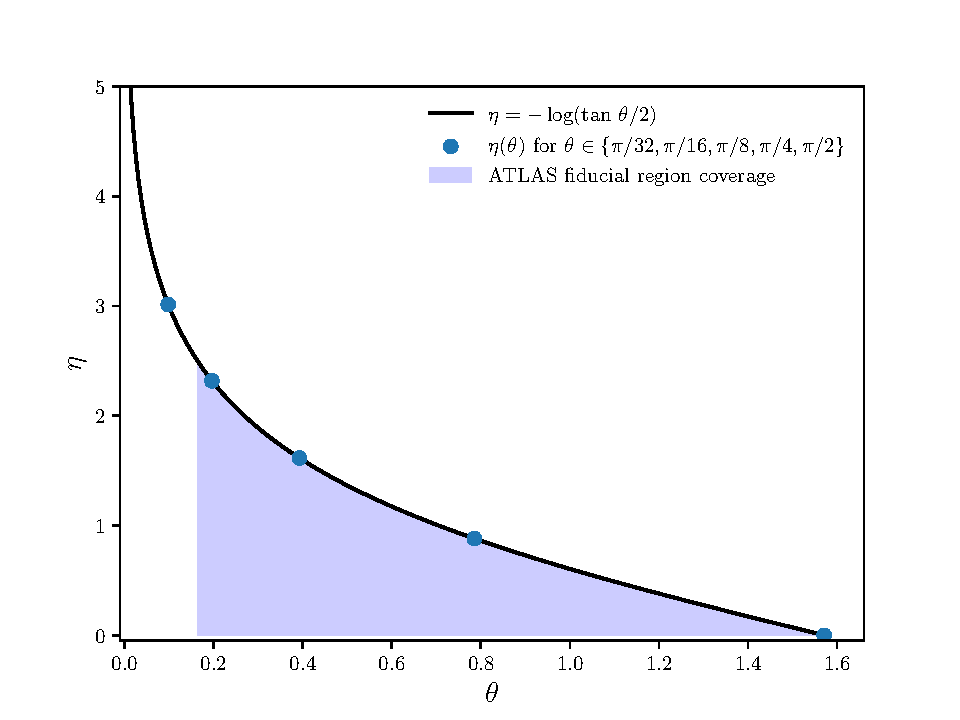
\includegraphics[width=0.8\linewidth]{preface/pseudorapidity.pdf}
 \caption[Pseudorapidity as a function of the polar angle.]{%
  Pseudorapidity, $\eta = - \ln \left(\tan \frac{\theta}{2}\right)$, as a function of the polar angle, $\theta$.
  The example markers are the points given in \Cref{table:pseudorapidity_angles}.
  The blue shaded region indicates the polar angle coverage up to $\eta = 2.5$, which is the end of the fiducial region coverage by the ATLAS inner detector.}
 \label{fig:pseudorapidity_angles}
\end{figure}

\section{Statistics}\label{section:statistics}

Statistics in particle physics

\subsection{Intervals and limits}\label{section:intervals_and_limits}

In addition to point estimates that determine an estimator, $\hat{\theta}$, of a parameter $\theta$, interval estimates give statistical precision to the measured value.
A common example of such an interval estimate is the set of points bounded by the point estimate and the estimated standard deviation: $\left[\hat{\theta} - \sigma_{\hat{\theta}}, \hat{\theta} + \sigma_{\hat{\theta}}\right]$.
The following is a short discussion of the construction, interpretation, and use of these intervals in the frequentist and Bayesian paradigms.

\subsubsection{Frequentist Confidence Intervals}

In the frequentist paradigm, a $1-\alpha$ confidence level (CL) confidence interval (CI) is an interval estimate that covers the true value of the parameter, $\theta$, $1-\alpha$ of the time it is constructed.
So the $95\%$ confidence level confidence interval covers the true value $95\%$ of the time it is constructed.
The method for constructing confidence intervals is called the ``Neyman Construction''~\cite{Neyman:1937uhy}, and results from inverting hypothesis tests.
This confidence interval construction can be described as a random variable that is the set of parameter points, $\left\{\vec{\theta}\right\}$, where the null hypothesis of each parameter point $\theta$ is accepted, $p\left(t > k_{\alpha}\middle| \theta\right) < \alpha$,

\begin{equation}
 \mathrm{CI}_{1-\alpha} = \left\{\vec{\theta}\,\middle| \,p\left(t > k_{\alpha}\middle| \vec{\theta}\right) < \alpha\right\}\,.
 \label{eq:confidence_interval}
\end{equation}

By construction, a hypothesis test of size $\alpha$ should accept the null hypothesis, given that the null is true, $(1-\alpha)$ of the time~\cite{Cranmer:2015nia}.\\

It is very important to take care in interpreting the meaning of the confidence interval, as it is often misunderstood and misused in analysis.
The confidence interval is constructed from the observed data%
\footnote{The data are a random variable in the frequentist paradigm.}
and so is a random variable and reflects information regarding the constructed estimator --- not the true parameter.
The confidence interval does \emph{not} give the interval in which there is a $1-\alpha$ probability of finding the true parameter value.
This is manifestly Bayesian and in fact is the interpretation of a Bayesian credible interval.
Keeping the definition of frequentist probability tightly in mind, the confidence interval should be interpreted as an interval of parameter values that $1-\alpha$ \emph{of the times is is constructed} contains the true parameter value.
Given this, in the frequentist paradigm one is \emph{unable} to make any statement on the probability that the true parameter value is contained in any specific confidence interval beyond the tautology that the true parameter is either contained in the it or it is not.
Any misuse of this result is not from a failing of the paradigm, but a misplaced desire of the analyst to have different questions answered than were asked.\\

In terms of computing a confidence interval, from observations that are governed by $\theta$ a test statistic, $t$, that is an estimator of $\theta$ is constructed.
For each value of the parameter to be tested, there exists an interval $\left[t_{1}, t_{2}\right]$ such that the probability of $t \in \left[t_{1}, t_{2}\right]$ is
\begin{equation}
 p\left(t_{1} < t < t_{2}\middle|\theta\right) = \int\limits_{t_{1}}^{t_{2}} f\left(t\middle|\,\theta\right)\,dt = 1-\alpha\,.
 \label{eq:confidence_interval_coverage}
\end{equation}
This interval represents a constant line segment in the $\left(t, \theta\right)$ parameter space plane at the given value of $\theta$.
By repeating this procedure for every value of $\theta$ to be tested, a band of line segments --- a ``confidence belt'' --- is created that is bound between the curves $\theta\left(t_{1}\right)$ and $\theta\left(t_{2}\right)$, as shown in the example in \Cref{fig:confidence_belt}.
Then, for any given observed value of the test statistic, $t'$, a boundary at $t = t'$ can be drawn in the plane that intersects the confidence belt at the points $\left(t', \theta_{2}\right)$ and $\left(t', \theta_{1}\right)$.
This resulting range of parameter values $\left[\theta_{1}, \theta_{2}\right]$ is the confidence interval~\cite{Cranmer:2015nia,PDG2018:Ch39}.\\

\begin{figure}[htbp]
 \centering
 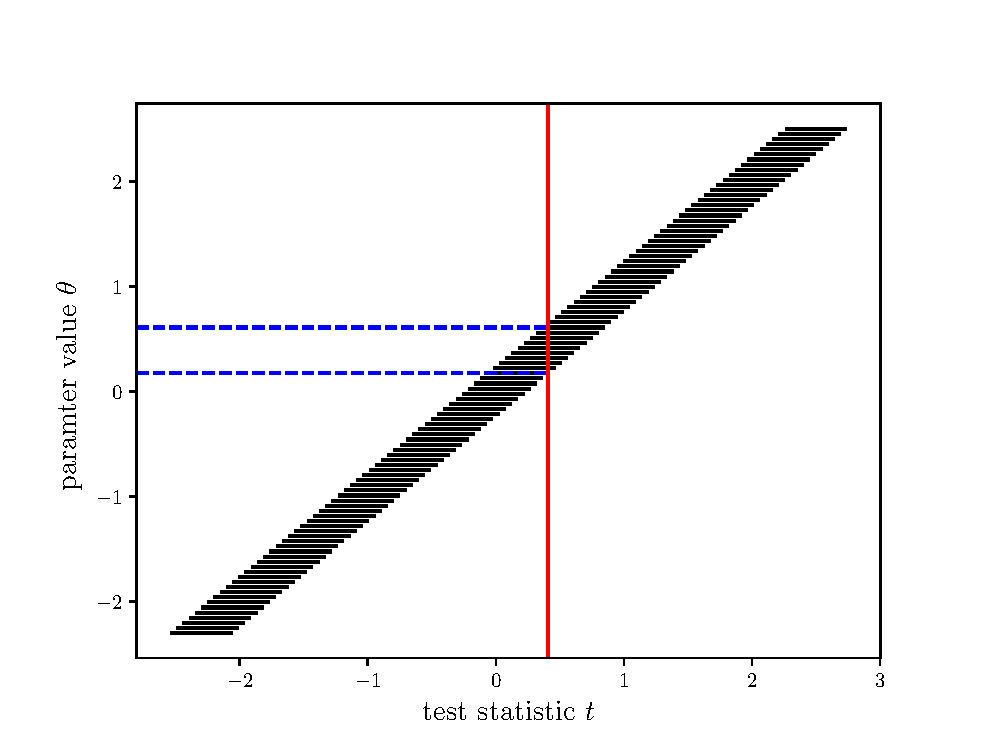
\includegraphics[width=0.4\linewidth]{preface/confidence_belt.eps}
 \caption{Example sketch of the construction of a confidence belt showing an observation in red intersecting the belt and the corresponding confidence interval as the parameter values bounded between the two blue dashed lines.}\label{fig:confidence_belt}
\end{figure}

The conditions of coverage from \Cref{eq:confidence_interval_coverage} do not uniquely specify $t_{1}$ and $t_{2}$, which allows for analysis specific choices to be made.
If central intervals are chosen, then the probabilities excluded below $t_{1}$ and $t_{2}$ are both $\alpha/2$.
In the event that only an upper (or lower) limit is of interest, as is common in searches for new physics where no excess has been observed, then the probability excluded below $t_{1}$ (or above $t_{2}$) is zero.
Alternatively, if the test statistic used is based on the likelihood ratio
\[
 \lambda = \frac{L\left(\theta\middle|\, t\right)}{L(\hat{\theta}|\, t)},
\]
the test statistic can be profiled to determine the range $\left[t_{1}, t_{2}\right]$.
Using such a test statistic results in the Feldman-Cousins confidence intervals~\cite{Feldman:1997qc}.\\

As the confidence interval can be a difficult concept to describe, a simple illustrative example follows.
Consider $n$ observations $\vec{x} = \left\{x_{1}, \cdots, x_{n}\right\}$ that are drawn from a Normal distribution with unknown mean $\theta$ and width $\sigma_{\theta}$.
This results in a sample mean $\hat{\theta}$ and standard deviation $\sigma_{\hat{\theta}}$.
To construct a $95\%$ confidence level central confidence interval for $\theta$, the test statistic $t = \left(\hat{\theta} - \theta\right)/\sigma_{\hat{\theta}}$ can be used such that ${p\left(t_{1} < t < t_{2}\middle|\theta\right) = 0.95}$, where $t_{1}$ and $t_{2}$ are respectively the $2.5$th percentile and $97.5$th percentile%
\footnote{$t_{1} = \mathrm{CDF}^{-1}\left(\alpha/2\right)$ and $t_{2} = \mathrm{CDF}^{-1}\left(1 - \alpha/2\right)$.}
of the Student's $t$-distribution for $n-1$ degrees of freedom, mean $\mu=\hat{\theta}$ and standard deviation $\sigma=\sigma_{\hat{\theta}}$.
Transforming the Student's $t$-distribution by $t' = \left(t-\hat{\theta}\right)/\sigma_{\hat{\theta}}$ to have $\mu=0, \sigma=1$ simplifies to ${p\left(-d < t' < d\middle|\theta\right) = 0.95}$.
Transforming to parameter space, ${p\left(\hat{\theta} - d\, \sigma_{\hat{\theta}} < \theta < \hat{\theta} + d\, \sigma_{\hat{\theta}}\right)  = 0.95}$, this gives a confidence interval of $\left[\hat{\theta} - d\, \sigma_{\hat{\theta}}, \hat{\theta} + d\, \sigma_{\hat{\theta}}\right]$.
Confidence intervals following this example construction are simulated and shown in \Cref{fig:confidence_intervals}.

\begin{figure}[htbp]
 \centering
 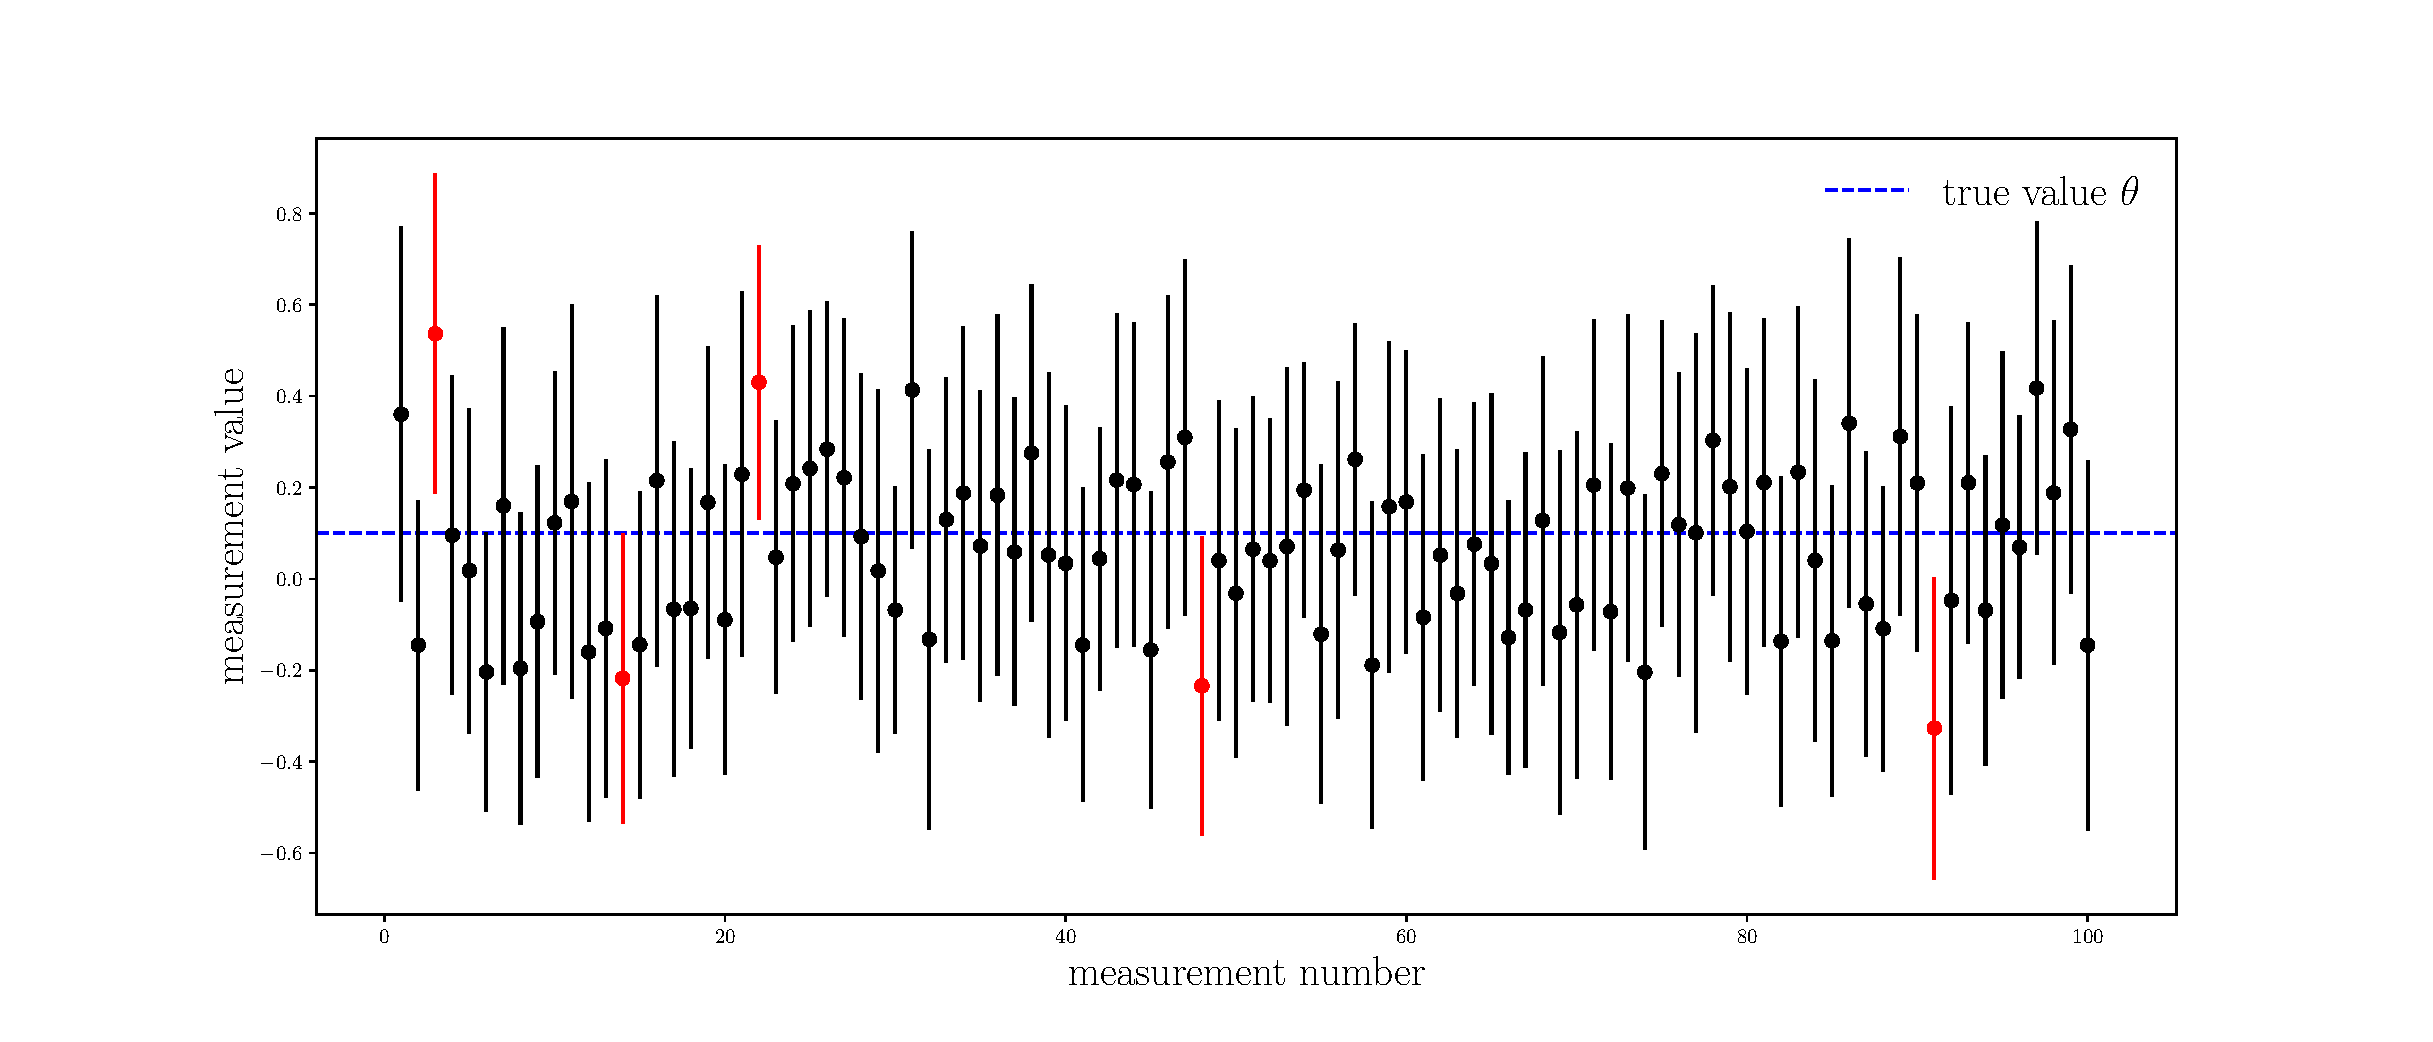
\includegraphics[width=\linewidth]{preface/confidence_intervals.eps}
 \caption{An example of 100 point estimates and associated $95\%$ confidence level confidence intervals of parameter value $\theta$.
  Confidence intervals that do not include the true value $\theta$ (dashed blue line) are colored red.}
 \label{fig:confidence_intervals}
\end{figure}

\subsubsection{Bayesian Credible Intervals}

In the Bayesian paradigm, a $1-\alpha$ credibility level (CL) credible interval (CI)%
\footnote{CL and CI are used for abbreviations for both the frequentist and Bayesian intervals.
 It will be made clear to the reader from context which paradigm is being considered.}
is an interval estimate where there is a $1-\alpha$ probability of containing the true parameter value --- which is a random variable.
As a result, it is simply the interval of the posterior predictive distribution $\left[\theta_{1}, \theta_{2}\right]$ that when integrated over gives a probability of $1-\alpha$,

\begin{equation}
 p\left(\theta_{1} < \theta < \theta_{2}\middle|\vec{x}\right) = \int\limits_{\theta_{1}}^{\theta_{2}} p\left(\theta\middle|\,\vec{x}\right)\,d\theta = 1-\alpha\,.
 \label{eq:credible_interval_coverage}
\end{equation}

As in the frequentist paradigm, there are different ways to select the credible interval range.
One can choose the shortest interval,%
\footnote{For a unimodal distribution this interval is known as the highest posterior density interval (HPD).}
the interval where probabilities excluded below $\theta_{1}$ and above $\theta_{2}$ are both $\alpha/2$ (this interval includes the median), the interval centered at the mean of the posterior (if the mean exists), or the intervals corresponding to upper (or lower) limits which reduce \Cref{eq:credible_interval_coverage} to the CDF (or CCDF) of $\theta$.\\

As a final word on interval estimates, it is worth remembering that the frequentist and Bayesian paradigms address different questions and so make different statements with their intervals.
\begin{itemize}
 \item Frequentist: When a confidence interval is constructed on future data, the constructed interval will contain the true parameter value with a probability (frequency) of $1-\alpha$.
 \item Bayesian: Given the observed data, there is a $1-\alpha$ probability that the true parameter value is contained by the constructed credible interval.
\end{itemize}


\section{Open Source Tools}\label{section:open_source}

This thesis and the researched described in it were made possible only through use of open source software.
The analysis was written in the open source languages \texttt{C++} and \texttt{Python} and made extensive use of the \texttt{ROOT} data analysis framework.
Similarly, parts of the analysis were conducted in Python and leveraged the SciPy ecosystem, most notably the NumPy and matplotlib libraries.
Additionally, the Keras library was used to interface with the TensorFlow machine learning framework for parts of the analysis.
The thesis itself was written in \LaTeXe, built using \texttt{latexmk} and \texttt{Make}, and versioned with Git.
Scientific research is built upon the open source community and tools, and this work would not have been made possible without it.


 \chapter{Introduction}\label{chapter:introduction}

The discovery of a Higgs-like boson~\cite{Higgs:1964ia,Higgs:1964pj,Higgs:1966ev,Englert:1964et,Guralnik:1964eu} at CERN in 2012 by the \Gls{ATLAS} and CMS collaborations~\cite{Aad:2012tfa,Chatrchyan:2012xdj} was a major triumph for both theoretical and experimental particle physics.
However, the properties of the new particle remain to be fully verified and the agreement of the predictions of the physics of the Higgs field by the \Gls{Standard Model} (SM) with observations of Nature require further testing.
One important property is the coupling strength of the the Higgs boson to bottom quarks $\left(\Hbb\,\right)$ --- this interaction was only experimentally observed in 2018 through associated production with a vector boson~\cite{Aaboud:2018zhk,CMS:2018abb}.
Additionally, there exist models of particle dark matter~\cite{Abdallah:2015ter} which include massive mediators between dark matter and Standard Model particles.
Such \gls{dark matter mediator}s (DMM) with couplings to Standard Model quarks would have the same decay signature to pairs of bottom quarks as the Higgs.
This thesis presents a search for low mass resonances, including Higgs, in the mass range of $100~\GeV$ to $200~\GeV$ with high momentum decaying to pairs of high momentum $b$-quarks with an associated jet $\left(\jXbb\,\right)$.
The goals of the search are to make a direct measurement of the couplings of Higgs to bottom quarks, and to search for evidence of exotic resonances with couplings to Standard Model quarks.
The thesis proceeds in the following manner.\\

\Cref{chapter:theory} introduces the field theories of the Standard Model, describes the physics of the Higgs field, and motivates the search for couplings of the Higgs to $b$-quarks and the search for exotic low mass resonances.
\Cref{chapter:LHC} introduces CERN's Large Hadron Collider and \Cref{chapter:ATLAS} describes the ATLAS experiment.
\Cref{chapter:bjet_trigger} describes the use of $b$-jet triggers in ATLAS for rapid identification of physics events with $b$-hadrons in the final state.
\Cref{chapter:event_reconstruction} gives an overview of the techniques used by the ATLAS collaboration to reconstruct the signature of particles in the ATLAS detector for physics quality data.
\Cref{chapter:analysis} is devoted to the application of the previous chapters in a search for boosted low mass resonances with a $b\bar{b}$ final state.
The results of this analysis are presented in \Cref{chapter:results}.
\Cref{chapter:software} gives a high level overview of general use statistical analysis software that was developed during the course of the analysis.
Finally, \Cref{chapter:conclusions} provides a summary of the state of measurements of Higgs couplings to heavy flavor quarks and the search for low mass exotic resonances given the results of the search, as well as an outlook to physics in Run 3 of the LHC.


 \StartAppendix%

 \chapter{The ATLAS Detector}\label{appendix:ATLAS_detector}

Appendix text goes here.


 % Bibliography goes below
 % Check with specific department on the appropriate
 % bibliography style to use

 \nocite{*}
 \bibliographystyle{bib/uiuchept}
 \raggedright
 \bibliography{bib/Luminosity,bib/Higgs}

\end{thesis}
\end{document}
